\documentclass[a4paper]{article}
\usepackage{hyperref}
\usepackage{amsmath,amssymb,amsthm, amsfonts}
\usepackage{tikz}
\usepackage{amsthm}
\usepackage{float}
\usepackage{algorithm}
\usepackage{algpseudocode}
\usepackage{hyperref}
\usepackage{listings}
\usepackage{comment}
\usepackage{pgfplots}
\usetikzlibrary{calc,trees,positioning,arrows,chains,shapes.geometric,%
    decorations.pathreplacing,decorations.pathmorphing,shapes,%
    matrix,shapes.symbols, decorations.markings}

\title{Models Used in Areas Affected by Memory}
\author{Jan Papou\v{s}ek}

\begin{document}
\maketitle

\subsection{Recall}

The basic concept used during solving tasks from \url{http://slepemapy.cz} is well-known as a recall.
Recall is one of the three core processes of memory, along with \textit{encoding} and \textit{storage}. A subject (student)
tries to retrieve information from the past. There are three types of racall:

\begin{description}
	\item[free]		A subject is given a list of items to remember and then is asked to recall
								them at any order.
	\item[serial] The ability to recall a list of items in the order which they occurred.
	\item[cued]		A participant is given a list of pairs, usually words and then is tested
								with one item	from the pair to recall the other.
\end{description}

In the context of learning a new language and vocabulary (which is related to \url{http://slepemapy.cz})
serial and cued recall is important. The serial recall plays a role in building sentences and cued
recall in translating a word from one language to another one.

\subsection{Forgetting Curve and Related Effects}

The recall probability is natuarally related to the forgetting in time $t$. The process can be
simplified by Equation \ref{eq:forgetting} where the parameter $s$ stands for the speed of forgetting.

\begin{align}
\label{eq:forgetting}
P_{recall} = e^{-\frac{t}{s}}
\end{align}

In addition to forgetting there are three other effects influecing the ability to memorize facts:

\begin{description}
	\item[repetition] The recall probability is higher with the larger number of student-task
										interactions.
	\item[lag]	There is a difference between interactions in one time and interactions spread over
							the nonzero time interval.
	\item[spacing]	The recall probability is dependent on time intervals amont the student-task
									interactions.
\end{description}

\begin{figure}[H]
\begin{center}
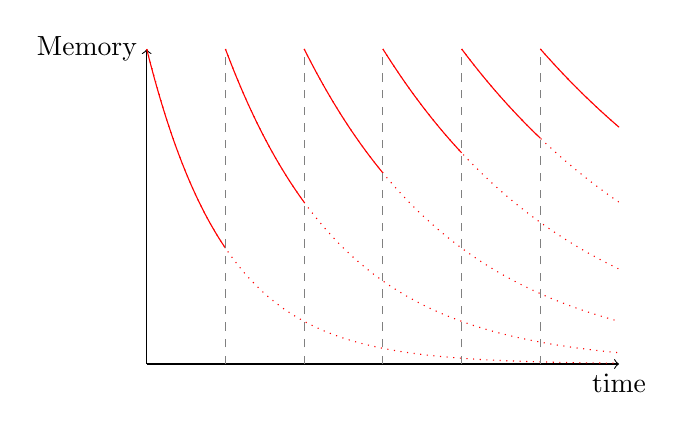
\begin{tikzpicture}
% horizontal axis
\draw[->] (0,0) -- (6,0) node[anchor=north] {time};
% vertical axis
\draw[->] (0,0) -- (0,4) node[anchor=east] {Memory};

% sigmoid curve
\draw[scale=1,domain=0:1,smooth,variable=\x,red] plot ({\x},{4 * exp((-\x/1))});
\draw[scale=1,domain=1:2,smooth,variable=\x,red] plot ({\x},{4 * exp((-(\x - 1)/1.5))});
\draw[scale=1,domain=2:3,smooth,variable=\x,red] plot ({\x},{4 * exp((-(\x - 2)/2))});
\draw[scale=1,domain=3:4,smooth,variable=\x,red] plot ({\x},{4 * exp((-(\x - 3)/2.5))});
\draw[scale=1,domain=4:5,smooth,variable=\x,red] plot ({\x},{4 * exp((-(\x - 4)/3))});
\draw[scale=1,domain=5:6,smooth,variable=\x,red] plot ({\x},{4 * exp((-(\x - 5)/3.5))});


\draw[scale=1,domain=0:6,smooth,variable=\x,red, dotted] plot ({\x},{4 * exp((-\x/1))});
\draw[scale=1,domain=1:6,smooth,variable=\x,red, dotted] plot ({\x},{4 * exp((-(\x - 1)/1.5))});
\draw[scale=1,domain=2:6,smooth,variable=\x,red, dotted] plot ({\x},{4 * exp((-(\x - 2)/2))});
\draw[scale=1,domain=3:6,smooth,variable=\x,red, dotted] plot ({\x},{4 * exp((-(\x - 3)/2.5))});
\draw[scale=1,domain=4:6,smooth,variable=\x,red, dotted] plot ({\x},{4 * exp((-(\x - 4)/3))});
\draw[scale=1,domain=5:6,smooth,variable=\x,red, dotted] plot ({\x},{4 * exp((-(\x - 5)/3.5))});

% task interaction
\draw[dashed, gray] (1,0) -- (1,4);
\draw[dashed, gray] (2,0) -- (2,4);
\draw[dashed, gray] (3,0) -- (3,4);
\draw[dashed, gray] (4,0) -- (4,4);
\draw[dashed, gray] (5,0) -- (5,4);

\end{tikzpicture}
\end{center}
\caption{Forgetting curves with decreasing speed for the repeatedly memorized fact.}
\end{figure}

\subsection{ACT-R}

To describe aspects of interaction between students and tasks requiring memorizing one can use a method
introduced by \cite{Pavlik2005} which is based on Adaptive Control of Thouht -- Rational (ACT-R) model.
ACT-R consists of a skill $\theta$ assigned to each student and a difficulty $\tau$ and discrimination $s$
assigned to each task. The model assumes a student solving tasks in times $t_1, \ldots, t_n$ in past and
predicts  a recall probability $P_{recall}$. It doesn't distinguish between correct and incorrect solutions.

\begin{align}
P_{recall}(\tau) = \frac{1}{1 + e^{\frac{\tau - \theta}{s}}}
\end{align}

\begin{figure}[H]
\begin{center}
\begin{tikzpicture}
% horizontal axis
\draw[->] (0,0) -- (6,0) node[anchor=north] {$\theta$};
% vertical axis
\draw[->] (0,0) -- (0,4) node[anchor=east] {$P_{recall}(\theta)$};

% 50% prob
\draw[dotted] (3,0) -- (3,2);
\draw[dotted] (0,2) -- (3,2);
\draw (3,0) node[anchor=north] {$\tau$};
\draw (0,2) node[anchor=east] {$\frac{1}{2}$};

% sigmoid curve
\draw[scale=1,domain=0:6,smooth,variable=\x,red]  plot ({\x},{4 * (1/(1 + exp(3- \x)))});

% discrimination arrow
\draw[->, >=stealth]  (2.5, 1.8) -- (3,2.3);
\draw (2.65, 2.05) node[anchor=south] {$s$};

\end{tikzpicture}
\end{center}
\label{actr}
\caption{Sigmoid curve describing probability predicted by ACT-R model.}
\end{figure}

\subsubsection{Basic Version}

It's natural to assume the more past interaction with task has a lower impact on a student's skill
than the more recent one. The basic version of model expresses a student's skill as a sum of
inversed times.

\begin{align}
\tau_n(t_1, \ldots, t_n) = \log\left(\sum_{i=1}^{n} t_i^{-d} \right)
\end{align}

This model somehow covers forgetting, but it doesn't deal with spacing effect.

\subsubsection{The First Attempt to Cover Spacing Effect}

To simplify spacing effect the second model assumes the effect is important mainly for the last to
solving times. Constant $d$ used to weigh times is replaced by a function containing $d_max$ parameter for
maximal value of $d_i$ and $b$ parameter expressing the influnce of the time.

\begin{align}
d_i = d(t_i, t_{i-1}) = \max\left(d_{max}, b \cdot (t_i - t_{i-1})^{-d}\right)
\end{align}

As the interval $[t_{i-1}, t_i]$ is longer, the value of the $d_i$ parameter is lower and $t_i^{d_i}$
has a higher impact on the final student's skill.

$$
t_i - t_{i-1} \uparrow~~\Longrightarrow~~d_i(t_i, t_{i-1})\downarrow~~\Longrightarrow~~t_i^{d(t_i, t_{i-1})} \uparrow
$$

Although the idea of counting only the last space is interesting, the \cite{Pavlik2005} shows the
model has a poor performance.

\subsubsection{The Second Attempt to Cover Spacing Effect}

To improve the prediction of the correct answer the model has to cover the spacing effect not only
for the last time interval, but also for the intervals before. To ensure this the third ACT-R based
model computes $d_i$ iterativaly with the knowledge of the previous student's skill.

\begin{align}
d_i(\theta_{i-1}) = c \cdot e^{\theta_{i-1}} + a
\end{align}

The student's skill for the first solving sessing is set to $-\infty$, so the $a$ parameter defines
value for $d_1$. The $c$ stands for the decay scale parameter.


\subsection{SAM}


\bibliographystyle{plain}
\nocite{*}
\bibliography{bibliography}

\end{document}
